\section{Solution Windows/DirectAccess}
La solution Windows repose sur DirectAccess.
DirectAccess est lié au rôle Remote Server dans Windows Server 2012 R2.
En bonne pratique, ce serveur Remote se place dans une DMZ.
Il va permettre de rediriger le trafic venant de l'extérieur vers l'intérieur. 

Les clients n'ont rien à faire de particulier, si ce n'est allumer leur machine.
En effet, dès que le système à charger les éléments réseau, il essaie d'établir la connexion vers le serveur Remote.
Ainsi l'utilisateur n'est pas dérangé, et a un accès direct aux ressources dont il a besoin.

\subsection{Schéma de l'infrastructure}
Le schéma est similaire à celui de la solution Juniper, à la différence que j'ai remplacé la passerelle SSL par le serveur Remote (Fig.\ref{fig:schemaDA} p.\pageref{fig:schemaDA}).

\begin{figure}[ht]
	\centering
	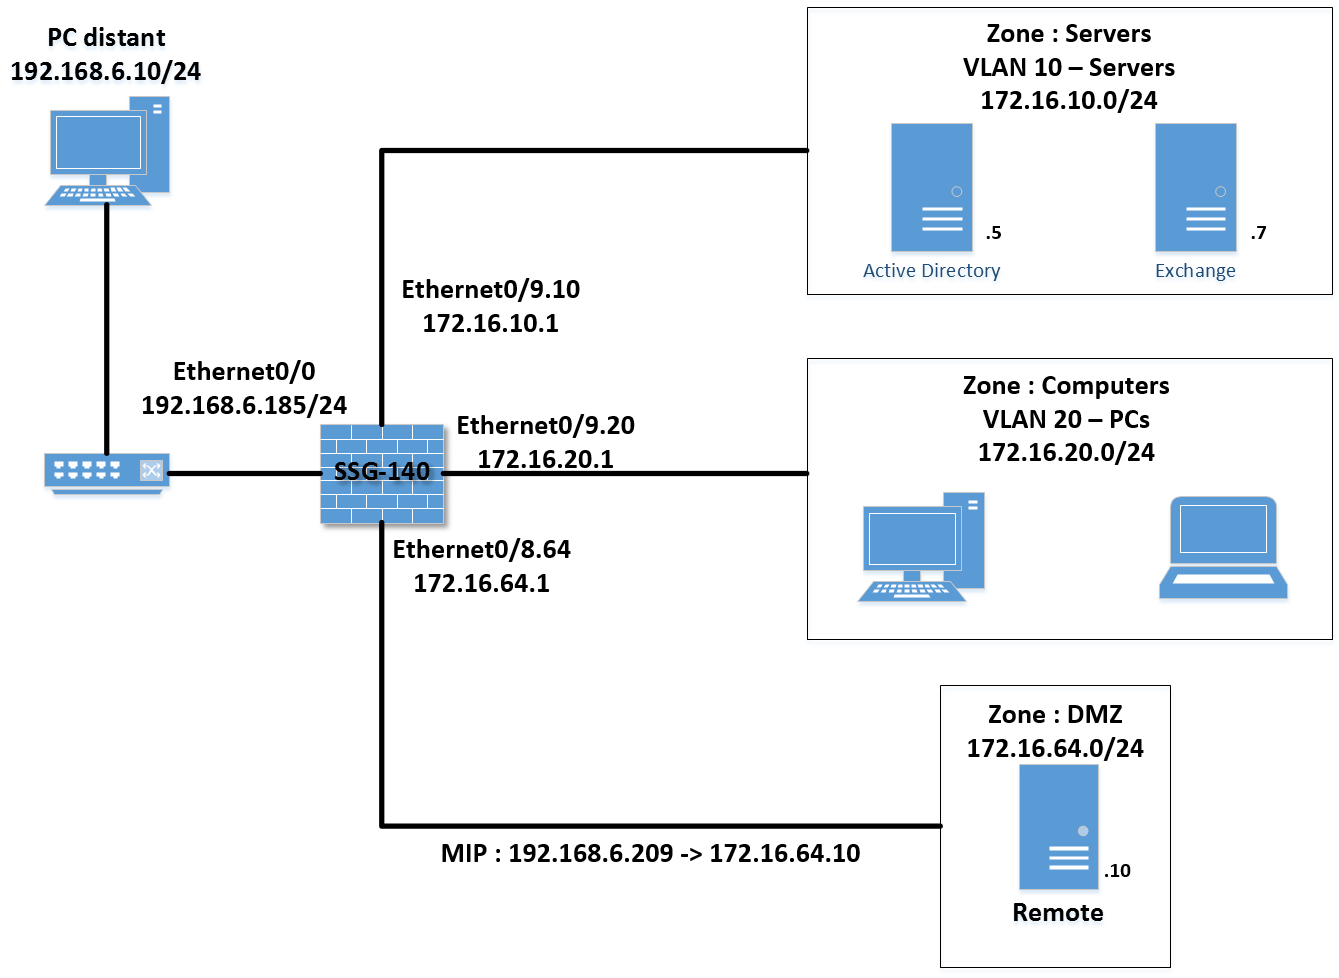
\includegraphics[width=16cm]{DA/schema.png}
	\caption{Schéma logique de l'infrastructure}
	\label{fig:schemaDA}
\end{figure}

\subsection{Configuration du serveur Remote}
Il suffit simplement d'ajouter le rôle "Remote Access" sur le serveur.
Ensuite, il faut suivre l'installateur du "Remote Access Management".

L'installateur demande juste des informations quant à l'adressage, l'emplacement du serveur.

En bonne pratique, il est conseillé de créer un groupe de sécurité spécifique pour les ordinateurs utilisant DirectAccess (voir Fig.\ref{fig:gsDA} p.\pageref{fig:gsDA}).
\begin{figure}[ht]
	\centering
	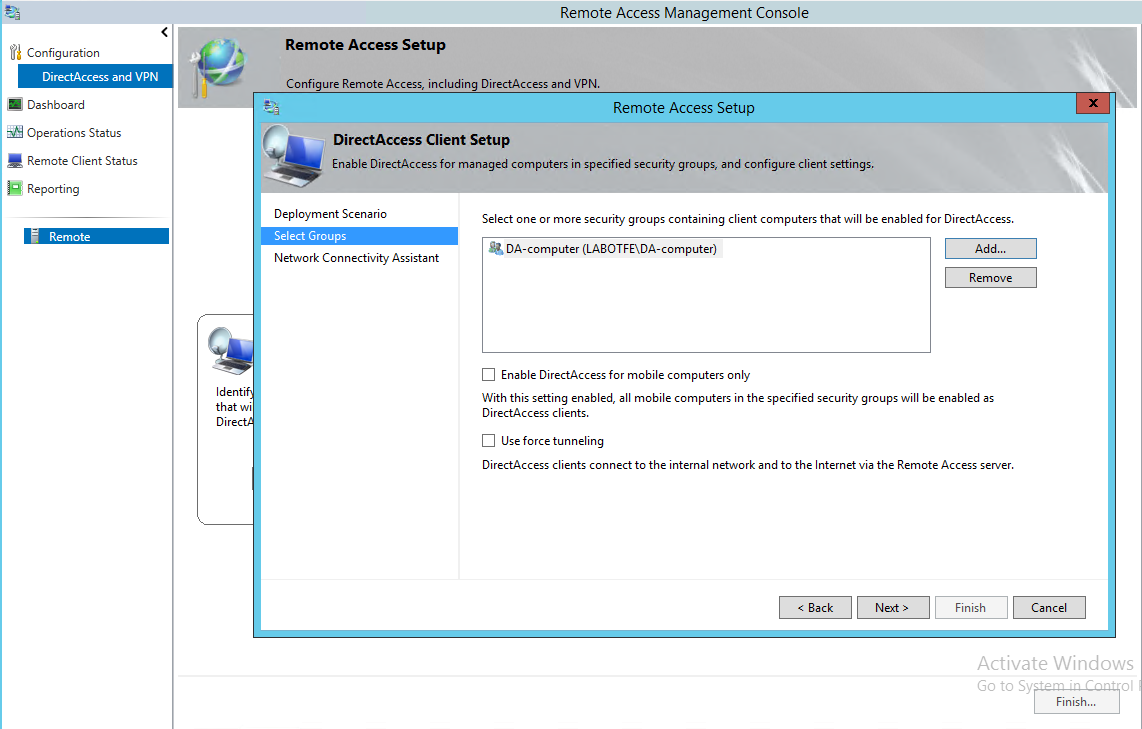
\includegraphics[width=16cm]{DA/DAGroup.png}
	\caption{Groupe de machines utilisant DirectAccess}
	\label{fig:gsDA}
\end{figure}
Par défaut, DirectAccess s'applique à toutes les machines du domaine.

DirectAccess s'applique aux machines via des GPOs, ce qui implique déjà que les machines sont membres du domaine.
De plus, DirectAccess ne fonctionne qu'avec des machines exploitant Windows 8(.1) Enterprise ou Windows 7 Enterprise/Ultimate.
Le serveur Remote crée deux nouvelles GPO voir Fig.\ref{fig:srvgpoDA} p.\pageref{fig:srvgpoDA} et Fig.\ref{fig:clientgpoDA} p.\pageref{fig:clientgpoDA}.
\begin{figure}[ht]
	\centering
	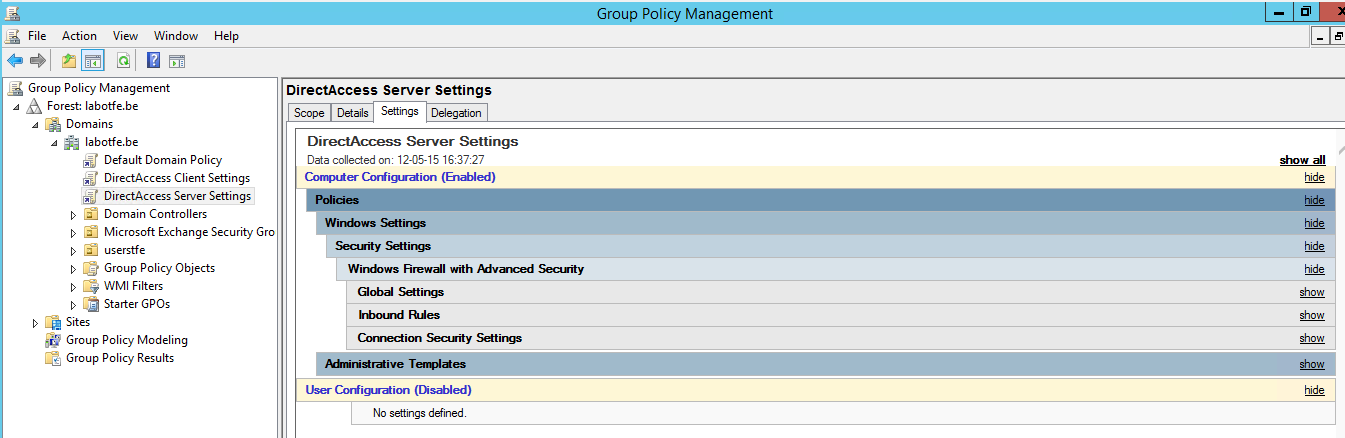
\includegraphics[width=16cm]{DA/DASrvGPO.png}
	\caption{GPO pour le serveur Remote}
	\label{fig:srvgpoDA}
\end{figure} 
\begin{figure}[ht]
	\centering
	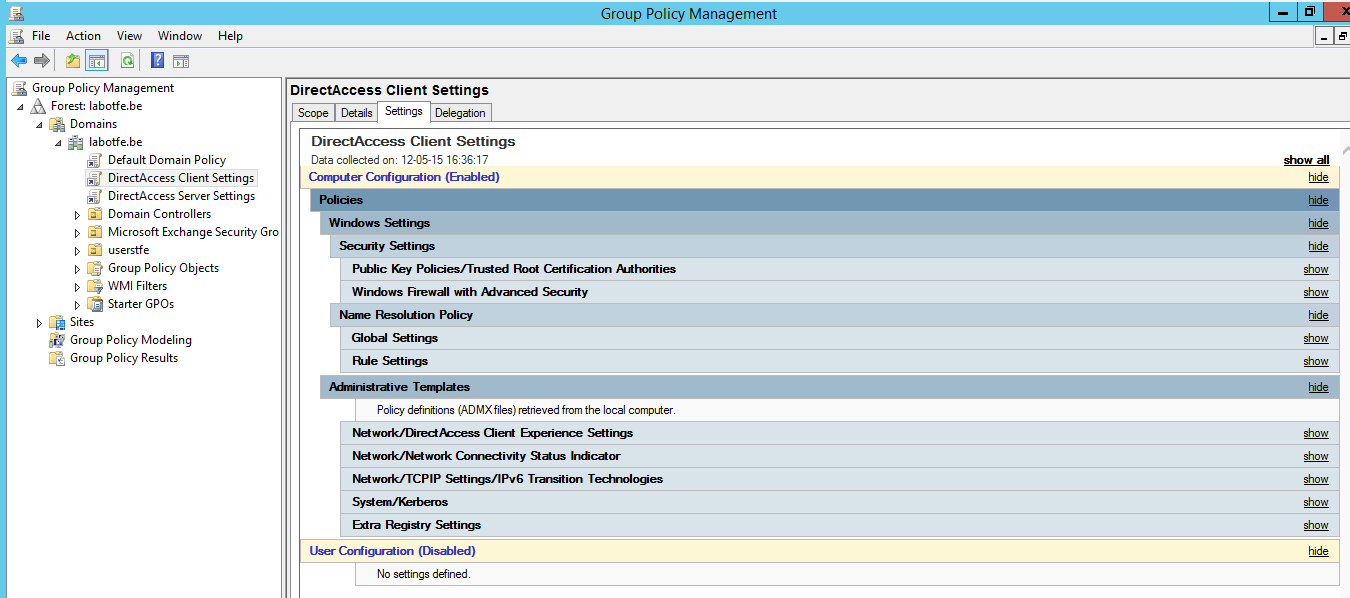
\includegraphics[width=16cm]{DA/DAClientGPO.png}
	\caption{GPO pour les machines clientes}
	\label{fig:clientgpoDA}
\end{figure} 

Pour savoir si la GPO pour les machines clientes est bien installée, il faut regarder les connexions de la machine.
Si la GPO est correctement ajoutée, un icône comme sur la Fig.\ref{fig:clientDA} p.\pageref{fig:clientDA} apparaît.
Dans ce cas, on voit même que la connexion au serveur Remote est réussie.
\begin{figure}[ht]
	\centering
	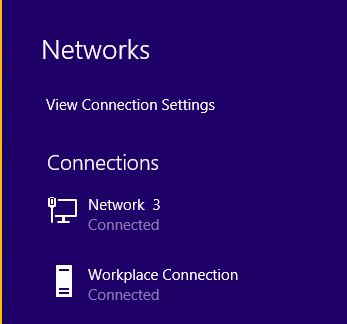
\includegraphics{DA/ClientConnexion.png}
	\caption{Vérification de la connexion sur une machine cliente}
	\label{fig:clientDA}
\end{figure} 